\newpage
\graphicspath{ {../choicungbi/domino2/} }

	{\textbf{\color{toancuabi} {Điểm thưởng}}   
	\vskip 0.1cm
	Khi chơi triomino ta có thể có điểm thưởng.  Để tìm hiểu luật thưởng điểm trước hết chúng mình sẽ  cùng tìm hiểu xem có thể có bao nhiêu quân triomino chung đỉnh. Em hãy quan sát Hình $5$ và trả lời câu hỏi $4$ dưới  đây nhé.
	\vskip 0.1cm
%	\begin{figure}[H]
%		\centering
%		\vspace*{-5pt}
%		\captionsetup{labelformat=empty, justification=centering}
%		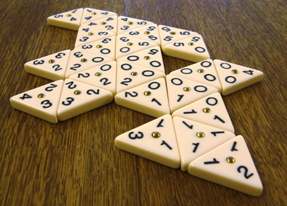
\includegraphics[width=0.34\textwidth]{h5a}
%		\caption{\textit{\small Hình 5}}
%	\vspace*{-15pt}
%	\end{figure}
	\textbf{\color{toancuabi}Câu hỏi $\pmb{3}$:}
	\vskip 0.1cm
	Có thể có nhiều nhất bao nhiêu quân triomino chung đỉnh?
	\vskip 0.1cm
	\hspace*{0pt}(A)  $2.$\hspace*{35pt}(B)  $3.$
	\hspace*{35pt}(C)  $4.$\hspace*{35pt}(D)  $5.$
	\hspace*{35pt}(E)  $6.$
	\vskip 0.1cm
	Theo luật của trò chơi Triomino, khi hoàn thành một nước đi hợp lệ, các em đã tạo thêm được trên “trận đồ” triomino ít nhất hai cặp đỉnh chạm nhau, mà hai số ở hai góc tại hai đỉnh cùng cặp là bằng nhau. Nói là ít nhất vì cũng có những lúc các em sẽ tạo thêm được trên “trận đồ” triomino ba hoặc bốn, hoặc thậm chí sáu cặp đỉnh chạm nhau, mà hai số ở hai góc tại hai đỉnh cùng cặp là bằng nhau. Chẳng hạn, nếu trước nước đi của các em, “trận đồ” triomino như ở Hình $9$ dưới đây và trong tay các em có quân triomino  $(3, 5, 5)$, thì bằng cách đặt quân triomino đó vào vị trí như ở Hình $10$, các em sẽ tạo thêm được ba cặp đỉnh chạm nhau, mà hai số ở hai góc tại hai đỉnh cùng cặp là bằng nhau.
	\begin{figure}[H]
		\centering
		\vspace*{-5pt}
		\captionsetup{labelformat=empty, justification=centering}
		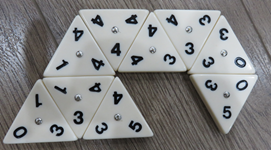
\includegraphics[height=0.2\textwidth]{h7a}\quad
		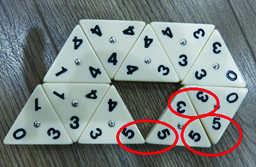
\includegraphics[height=0.2\textwidth]{h8a}
		\caption{\textit{\small Hình 9 \hspace*{75pt} Hình $10.$}}
		\vspace*{-10pt}
	\end{figure}
	Các em hãy tự nghĩ ra các tình huống mà sau một nước đi hợp lệ nào đó, người đi nước ấy sẽ tạo thêm được trên “trận đồ” \linebreak triomino bốn cặp đỉnh chạm nhau, hoặc sáu cặp đỉnh chạm nhau, mà hai số ở hai góc tại hai đỉnh cùng cặp là bằng nhau nhé.
	\vskip 0.1cm
	Tuy có thể xảy ra, nhưng thường thì rất hiếm khi gặp các tình huống như trên trong các cuộc chơi triomino. Vì thế, trong trò chơi Triomino, có luật thưởng điểm như sau:
	\vskip 0.1cm
	--\ Nếu sau một nước đi hợp lệ, có thêm ba cặp đỉnh chạm nhau, mà hai số ở hai góc tại hai đỉnh cùng cặp là bằng nhau, được tạo ra thì người đi nước ấy sẽ được thưởng thêm $40$ điểm;
	\vskip 0.1cm
	--\ Nếu sau một nước đi hợp lệ, có thêm một bộ sáu quân \linebreak triomino có chung đỉnh thì người đi nước ấy sẽ được thưởng thêm $50$ điểm;
	\vskip 0.1cm
	--\ Nếu sau một nước đi hợp lệ, có thêm hai bộ sáu quân triomino có chung đỉnh thì người đi nước ấy sẽ được thưởng thêm $60$ điểm.
	\vskip 0.1cm
	Ví dụ, người đã đặt quân triomino $(3, 5, 5)$ lên bàn chơi triomino để chuyển “trận đồ” ở Hình $9$ thành “trận đồ” ở Hình $10$ sẽ được nhận
	\vskip 0.1cm
	\hspace*{100pt}$3+5+5=13$ (điểm)
	\vskip 0.1cm
	từ nước đi hợp lệ đó, và đồng thời được thưởng thêm $40$ điểm, do đã tạo thêm được ba cặp đỉnh chạm nhau, mà hai số ở hai góc tại hai đỉnh cùng cặp là bằng nhau. Như vậy, sau nước đi hợp lệ ấy, người chơi sẽ cộng thêm được vào quỹ điểm của mình:
	\vskip 0.1cm
	\hspace*{100pt} $13+40=53$ (điểm).
	\vskip 0.1cm
	Hay như, sau khi đã đặt quân triomino $(4, 5, 3)$ lên bàn chơi \linebreak triomino để chuyển “trận đồ” ở Hình $9$ thành “trận đồ” ở Hình $10$ dưới đây, người đã đi nước đi hợp lệ ấy sẽ cộng thêm được vào quỹ điểm của mình:
	\vskip 0.1cm
	\hspace*{80pt} $(4+5+3)+50 =62$ (điểm).
	\begin{figure}[H]
		\centering
		\captionsetup{labelformat=empty, justification=centering}
		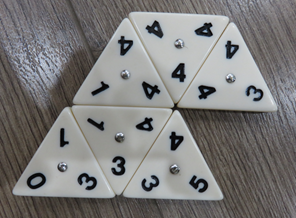
\includegraphics[height=0.3\textwidth]{h9a}
		%\caption{\textit{\small Hình 9}}
		%\captionsetup{labelformat=empty, justification=centering}
		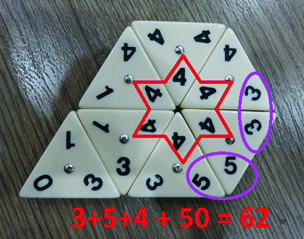
\includegraphics[height=0.3\textwidth]{h10a}
			\caption{\textit{\small Hình $9.$ \hspace*{75pt} Hình $10.$}}
		%\caption{\textit{\small Hình 10}}
		%\vspace*{-15pt}
	\end{figure}
	Còn sau khi đã đặt quân triomino $(4, 5, 3)$ lên bàn chơi triomino để chuyển “trận đồ” ở Hình $11$ thành “trận đồ” ở Hình $12$ dưới đây, người đã đi nước đi hợp lệ ấy sẽ cộng thêm được vào quỹ điểm của mình:
	\vskip 0.1cm
	\hspace*{40pt} $(4+5+3)+60=72$ (điểm).
	\vskip 0.1cm
	\begin{figure}[H]
		\centering
		\vspace*{-5pt}
		\captionsetup{labelformat=empty, justification=centering}
		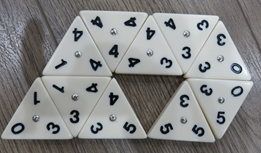
\includegraphics[height=0.25\textwidth]{h11a}\quad
		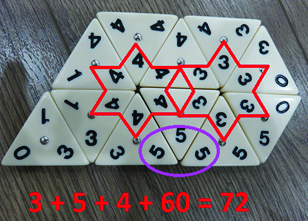
\includegraphics[height=0.25\textwidth]{h12a}
		\caption{\textit{\small Hình $11.$ \hspace*{75pt} Hình $12.$}}
		\vspace*{-5pt}
	\end{figure}
	Và bây giờ, để cảm nhận được một trong các lý do của sự hiếm gặp các tình huống nêu trên trong các cuộc chơi triomino, các em hãy trả lời Câu hỏi $5$ dưới đây nhé.
	\vskip 0.1cm
	\begin{multicols}{2}
		\textbf{\color{toancuabi}Câu hỏi $\pmb{4}$:}
		\vskip 0.1cm
		Em có thể đặt thêm hay không một quân  triomino vào “trận đồ” triomino ở Hình $13$, để có được một bộ sáu quân \linebreak triomino có chung đỉnh?		\begin{figure}[H]
			\centering
			%\vspace*{-5pt}
			\captionsetup{labelformat=empty, justification=centering}
			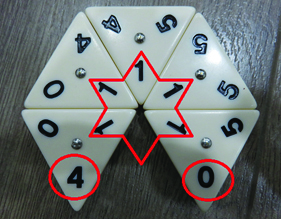
\includegraphics[width=0.34\textwidth]{h13a}
			\caption{\textit{\small Hình $13.$}}
			\vspace*{-5pt}
		\end{figure}
	\end{multicols}
	{\textbf{\color{toancuabi}\color{toancuabi} {Cùng chơi}}   
	\vskip 0.1cm
	Ở phần trước chúng mình đã tìm hiểu về cách đi, cách tính điểm và điểm thưởng của trò chơi Triomino. Trong phần  này, chúng mình sẽ rủ bàn bè cùng chơi nhé.
	\vskip 0.1cm
	Trò triomino có thể có nhiều người chơi, ở đây chúng ta tìm hiểu cách chơi với hai người chơi nhé. Hai người sẽ luân phiên nhau thực hiện các nước đi.
	\vskip 0.1cm
	Nếu một người nào đó, ở lượt của mình không muốn dùng quân triomino đang có trên tay để thực hiện nước đi hoặc không thể thực hiện nước đi do trên tay không có quân triomino phù hợp thì phải bốc một quân trong số các quân đang nằm sấp trên mặt bàn (nếu có). Sau khi bốc xong, nếu người đó vẫn không muốn thực hiện nước đi hoặc vẫn không thực hiện được nước đi thì gõ “cạch” một nhát xuống mặt bàn để chuyển tiếp lượt chơi cho người kia. Trường hợp cần bốc nhưng trên mặt bàn không còn quân nằm sấp nào, chỉ cần gõ “cạch” để chuyển tiếp lượt chơi. Mỗi lần bốc một quân triomino như thế, người bốc bị trừ $5$ điểm.
	\vskip 0.1cm
	Trong quá trình chơi, sẽ có một thời điểm xảy ra một trong hai tình huống sau:
	\vskip 0.1cm
	$\bullet$ \textit{Tình huống $1$: Lần đầu tiên trong quá trình chơi, có một người, ngay sau khi thực hiện xong nước đi của mình, trên tay không còn một quân triomino nào nữa.}
	\vskip 0.1cm
	$\bullet$ \textit{Tình huống $2$: Mọi người chơi đều còn quân trên tay, nhưng không một người nào có thể thực hiện nước đi, và đồng thời, trên mặt bàn không còn một quân nằm sấp nào.}
	\vskip 0.1cm
	Nếu tình huống $2$ xảy ra thì ván chơi được kết thúc ngay tại thời điểm xảy ra tình huống đó.
	\vskip 0.1cm
	Nếu xảy ra tình huống $1$ thì cuộc chơi sẽ được kết thúc ngay tại thời điểm đó, nếu người hết quân trên tay (được nói đến trong tình huống) là người chơi thứ hai. Trường hợp người hết quân trên tay là người chơi đầu tiên, người còn lại được chơi thêm một lượt  nữa. Đến đây ván chơi kết thúc. Luật này đảm bảo sự công bằng: hai bạn chơi được đi số lượt như nhau. Ngoài ra, bất cứ người chơi nào hết quân trên tay đều được cộng thêm $25$ điểm vào quỹ điểm của mình.
	\vskip 0.1cm
	Sau khi ván chơi kết thúc, điểm số của mỗi người chơi được tính như sau: Điểm số của ván chơi bằng số điểm đã tích lũy được trong quá trình chơi trừ đi tổng tất cả các số được ghi trên mặt của tất cả các quân mà người đó còn giữ trên tay (nếu có). Bạn nào có điểm cao hơn sẽ thắng ván chơi đó. 
	\vskip 0.1cm
	Cuối cùng là một câu hỏi dành cho các em:
	\vskip 0.3cm
	\textbf{\color{toancuabi}Bài tập:} Hai bạn Pi và Bi cùng chơi một ván triomino. Có một thời điểm mà “trận đồ” triomino trên bàn chơi như ở Hình $14$:
	\vskip 0.1cm
	\begin{figure}[H]
		\centering
		\vspace*{-5pt}
		\captionsetup{labelformat=empty, justification=centering}
		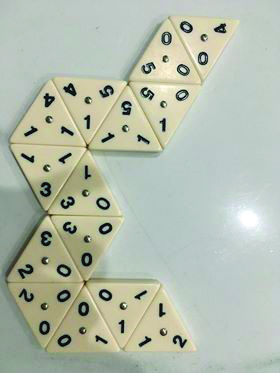
\includegraphics[height=0.3\textwidth,angle=90]{h9}
		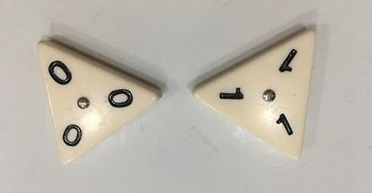
\includegraphics[height=0.225\textwidth]{h10}
		%\caption{\textit{\small Hình 10}}
		\caption{\textit{\small Hình $14.$ \hspace*{75pt} Hình $15.$}}
		\vspace*{-8pt}
	\end{figure}
	Biết rằng, trong số các quân triomino mà Pi cầm trên tay có quân $(0, 0, 0)$, còn trong số các quân triomino mà Bi cầm trên tay có quân $(1, 1, 1)$ (xem Hình $15$).
	\vskip 0.1cm
%	\begin{figure}[H]
%		\centering
%		\vspace*{-5pt}
%		\captionsetup{labelformat=empty, justification=centering}
%		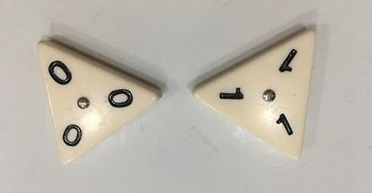
\includegraphics[scale=0.65]{h10}
%		\caption{\textit{\small Hình 10}}
%		\vspace*{-8pt}
%	\end{figure}
	Hỏi ván chơi nói trên của Pi và Bi sẽ kết thúc theo kiểu tình huống nào ($1$ hay $2$)? Vì sao?
	\begin{figure}[H]
	\centering
	\vspace*{-5pt}
	\captionsetup{labelformat=empty, justification=centering}
	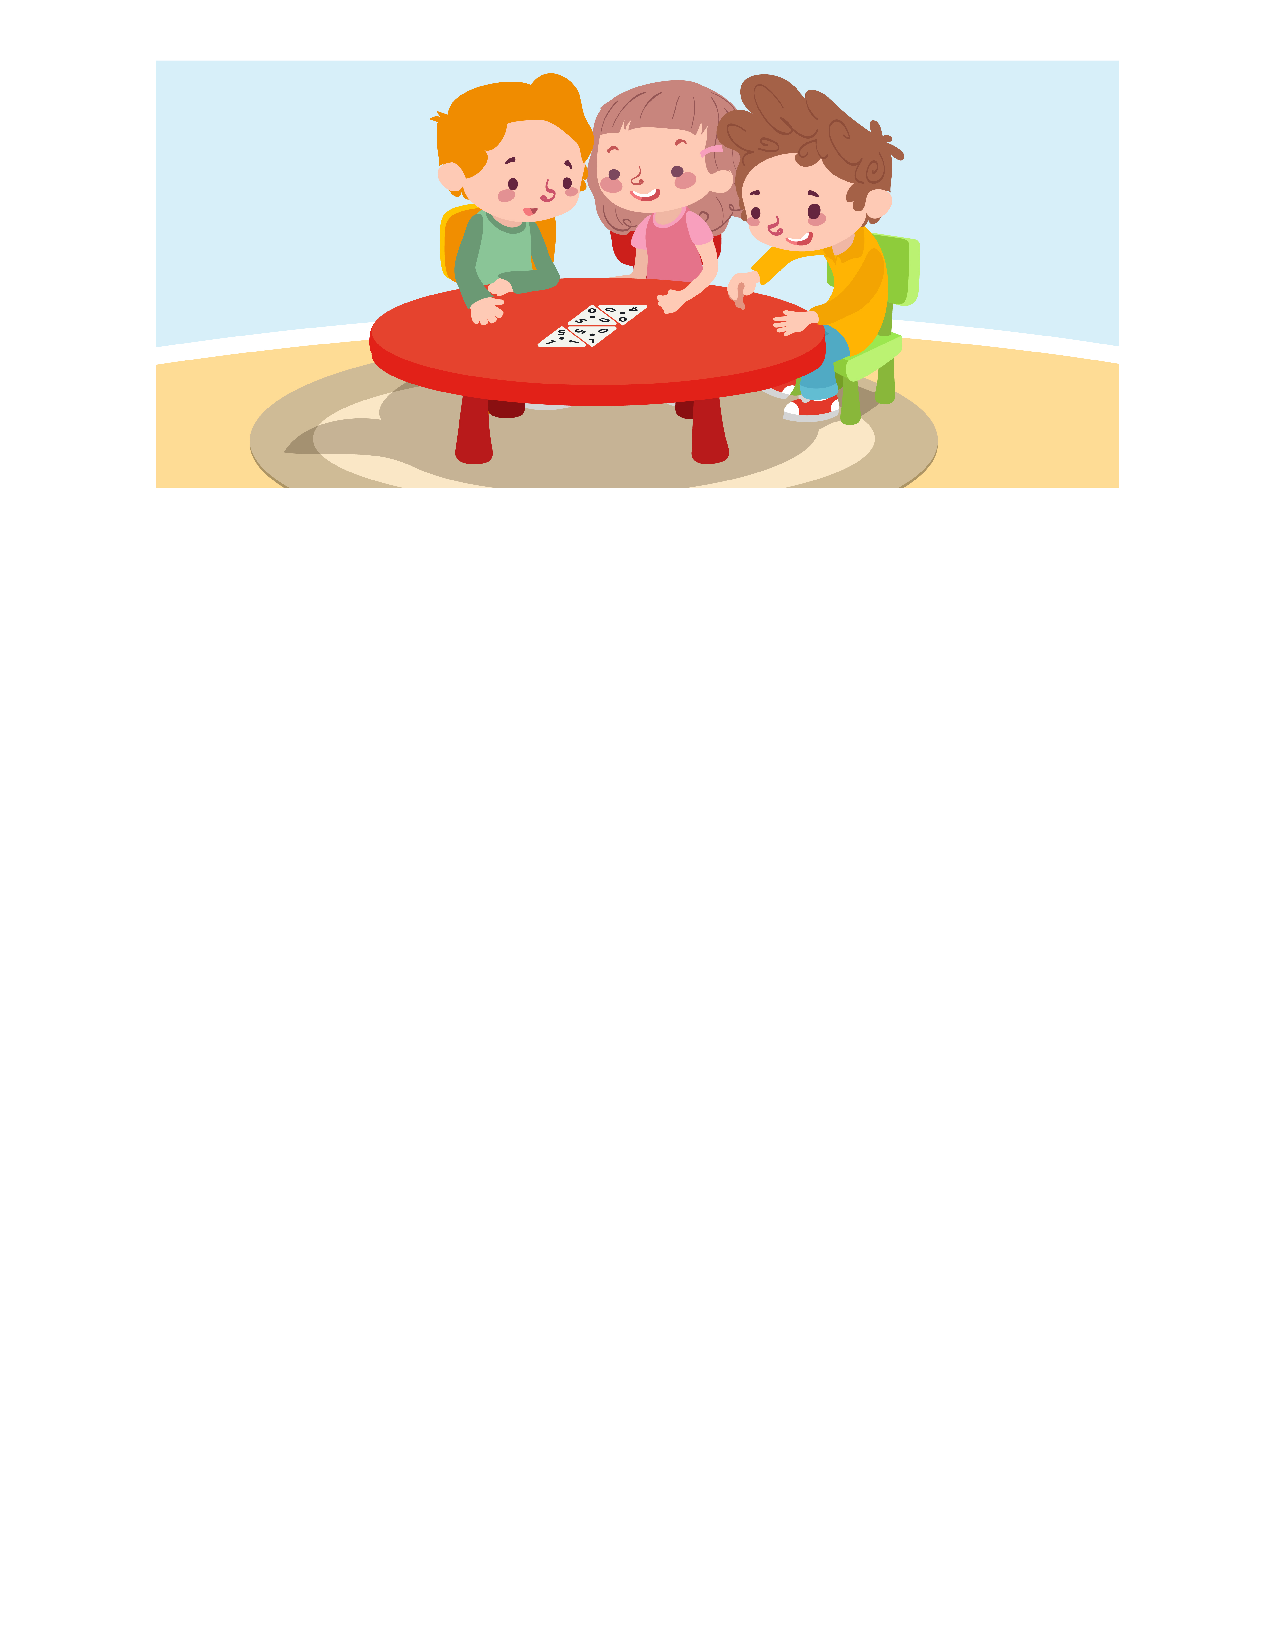
\includegraphics[width=1\textwidth]{h11}
	\vspace*{-20pt}
	\end{figure}
	Các em hãy đọc cách chơi triomino và rủ bạn chơi cùng mình nhé. 